\chapter{3D reconstruction} 
\label{Chap:3DReconstruction}

\subsection{Stereo-Reconstruction of Dense Surfaces}
% ~~~~~~~~~~~~~~~~~~~~~~~~~~~~~~~~~~~~~~~~~~~~~~~~~~~~~~~~~~~~~~~~~~~~~~~~~~~~~

To perform the dense reconstruction of the floor surface in front of the robot, we rely on a real-time approach similar to KinectFusion algorithm proposed in~\cite{Newcombe2011}. This approach, originally developed for a RGB-D sensor, models 3-D surfaces as zero-valued level sets of functions defined over the workspace volume. These functions are referred to as truncated signed distance function (TSDF) and they are built incrementally, by integrating the depth measurements the sensor provides, frame after frame. TSDF are defined in the 3D space, and their value is the signed distance to the closest obstacle. Here, we extend this approach, initially proposed for RGB-D depth data, to disparity data generated from a stereo head. Although the stereo data is noisier than the one from RGB-D sensors, it is a passive sensor and can be used outdoors in sunlight conditions.


Consider, as in the previous sections, that $k$ is a discretized time index. The idea is to update a mathematical representation of the surface through a volumetric TSDF model (defined over a 3D grid), referred to as $F_k$. The basic steps for integrating one new set of disparity measurements at time $k$, to update $F_k$ and the corresponding surface, are the following ones: (i) Filter the raw depth measurements generated from the stereo head, $D_k$; here we used bilateral filtering for that purpose; (ii) From these filtered measurements and the prediction of the estimated surface at the previous step, estimate the transformation between the measured surface and the predicted one using the iterative closest point algorithm (ICP) and update the camera pose; (iii) Compute a volumetric grid formed from ``local'' TSDF values $F_{D_k}$, to which confidence weights $W_{D_k}$ are associated, and integrate them into the global volumetric grid $\{F_k,W_k\}$; (iv) Predict a new surface for the next iteration by using ray-casting over the zero-crossings of the fused global volumetric grid $\{F_k,W_k\}$. 

The core of this algorithm is the computation and fusion of volumetric grids (i.e., the third step mentioned above). For a 3D point $\mathbf{p}$ expressed in the global frame $g$, its value in the current local volumetric grid $\{F_{D_k},W_{D_k}\}$ is computed as

$$
\left\{
\begin{array}{ccc}
F_{D_{k}}(\mathbf{p}) &=& \Psi (\lambda^{-1} \left \| \mathbf{t}_{g,k} - \mathbf{p}\right \| - D_k(\mathbf{x})), \\
W_{D_{k}}(\mathbf{p}) &\propto& \cos(\theta)/D_{k}(\mathbf{x}),
\end{array}
\right.
$$

with
$$
\Psi (\eta) =
\left \{
\begin{array}{cc}
\min(1,\frac{\eta}{\mu}) ~\text{sgn}(\eta) & \text{iff} ~ \eta \geq -\mu \\
\mbox{ null } & \mbox{ otherwise }
\end{array}
\right. , ~
\lambda = \left \| \mathbf{K}^{-1} [\mathbf{x}^\top 1]^\top \right \|,~
%\lambda = \left \| \mathbf{K}^{-1} \left[ \begin{matrix} \mathbf{x} \\ 1 \end{matrix} \right] \right \|,
$$

$\mu$ being a truncation distance (parameter of the algorithm), $\mathbf{x} = \pi([\mathbf{K},\mathbf 1] T^{-1}_{g,k} \mathbf{p}) \in \mathbb{R}^2$ being the image projection of $\mathbf p$. $\mathbf{K}$ is the $3\times 3$ matrix of intrinsic parameters of the camera, $\pi$ is the projection operator, $T_{g,k} = \left[ \begin{matrix} \mathbf{R}_{g,k} & \mathbf{t}_{g,k} \\ 0 & 1 \end{matrix} \right]$ the pose of the camera, at time $k$, in the global frame $g$, and $\theta$ the angle between the associated pixel ray direction and the surface normal.

The global volumetric grid at time $k$ is formed by the weighted average of all individual volumetric grids up to $k-1$. It can be shown that the optimal grid can be obtained incrementally using a simple point-wise on-line weighted average,

\begin{eqnarray*}
 F_k(\mathbf{p}) &=& \frac{W_{k-1}(\mathbf{p}) F_{k-1}(\mathbf{p}) + W_{D_{k}}(\mathbf{p}) F_{D_{k}}(\mathbf{p}) }{ W_{k-1}(\mathbf{p}) + W_{D_{k}}(\mathbf{p}) }, \\
 W_k(\mathbf{p}) &=& W_{k-1}(\mathbf{p}) + W_{D_{k}}(\mathbf{p}).
\end{eqnarray*}


To use this algorithm with stereo data and generate local data $D_k$, a disparity map from a pair of rectified images is estimated, from which the depth map $D_k$ is derived, supposing the stereo rig is completely calibrated. The literature of algorithms that estimate disparity maps is huge, but since a real time one is needed for this application, the one proposed in~\cite{Geiger2010} has been used. This algorithm estimates a piece-wise disparity map using an initial sparse disparity map of high textured points as vertices that define a triangulation of the image. Then, the dense disparity map of each sub-region is estimated by using the initial, sparse disparity map as a prior in a probabilistic scheme. The steps of the reconstruction process are illustrated in Fig.~\ref{Fig:Reconstruction}.

\begin{figure}[h]
\centering
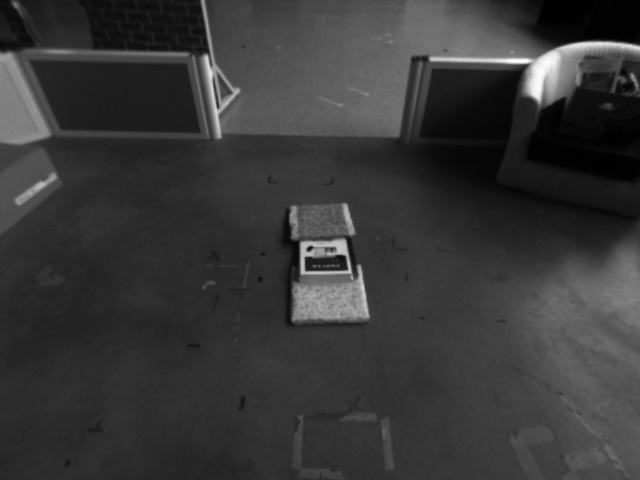
\includegraphics[scale=0.17]{figures/right0001}
\hspace{0.2cm}
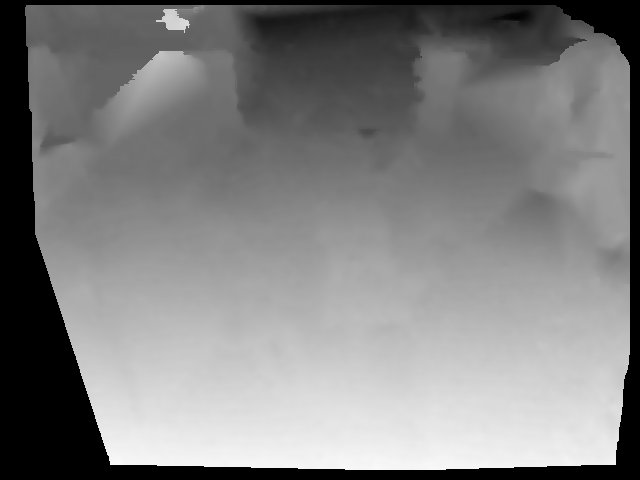
\includegraphics[scale=0.17]{figures/left0001_disp}
\hspace{0.2cm}
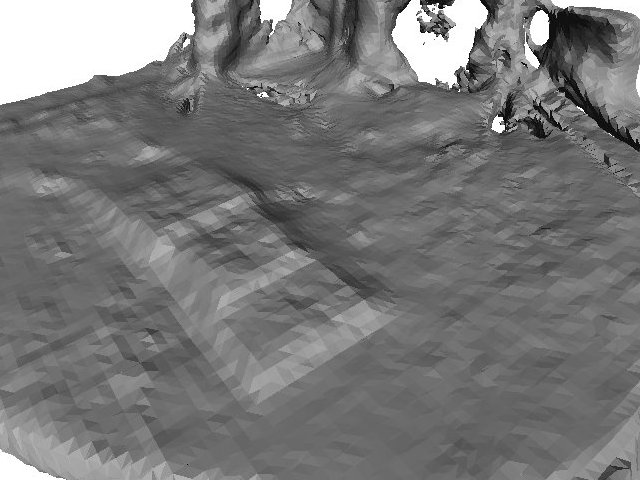
\includegraphics[scale=0.22]{figures/snapshot02}
\caption[]{From a pair of images of the scene in front of the robot (left) we estimate a dense disparity map (middle) and from this disparity map we estimate a dense surface integrating the previous frames into the volumetric grid.}
\label{Fig:Reconstruction}
\end{figure}
